\documentclass{article}
  \usepackage[a4paper,top=3cm,bottom=3cm,left=2.5cm,right=2.5cm,marginparwidth=1.75cm]{geometry}
  \title{Piano di Progetto}
  \usepackage[T1]{fontenc}
  %\usepackage{lmodern}
  \usepackage[utf8]{inputenc}
  \usepackage[italian]{babel}
  \usepackage{amsmath}
  \usepackage{graphicx}
  \usepackage{booktabs}
  \usepackage{longtable}
  \usepackage{wrapfig}
  \usepackage{mdframed}
  \usepackage{tcolorbox}
  \usepackage{xcolor}
  \usepackage{hyperref}
  \definecolor{ProcessBlue}{HTML}{00B0F0}
  
  %% HEADER
  \usepackage[sfdefault,lf]{carlito}
  %% The 'lf' option for lining figures
  %% The 'sfdefault' option to make the base font sans serif
  \usepackage[parfill]{parskip}
  \renewcommand*\oldstylenums[1]{\carlitoOsF #1}
  \usepackage{fancyhdr}
  %\usepackage{natbib}
  %\usepackage{authblk}
  \setlength{\headheight}{41pt}
  
  \fancyhead[L]{Piano di Progetto}
  \fancyhead[R]{
  
\includegraphics[width=4cm]{gfx/logo.pdf}
  }
  \pagestyle{fancy}
  \fancypagestyle{plain}{%
  \fancyhf{} % clear all header and footer fields
  \fancyfoot[C]{\sffamily\fontsize{9pt}{9pt}\selectfont\thepage} % except the center
  \renewcommand{\headrulewidth}{0pt}
  \renewcommand{\footrulewidth}{0pt}}
  %\pagestyle{plain}
  
  \makeatletter
  
  \newcommand{\spacedlowsmallcaps}[1]{\textbf{#1}}
  \newcommand{\titleColor}{}
  \makeatother
  
  \usepackage{graphicx}
  \usepackage[absolute]{textpos}
  
  \begin{document}
  \thispagestyle{empty}
  \setlength{\TPHorizModule}{1mm}
  \setlength{\TPVertModule}{1mm}
  
  \begingroup
    \fontsize{11pt}{11pt}\selectfont
    \linespread{1.05}
  
    \begin{textblock}{50}(0,0)
    \noindent \includegraphics{gfx/00_cafoscari}
    \noindent \end{textblock}
    ~
    \begin{textblock}{143}(47,42)
  
    \noindent {\LARGE{}Progetto per\\Ingegneria del Software \emph{(CT0090)}}\\
    \vspace{30pt}
    
    %\vspace{30pt}
  
  
    \noindent %
    \begin{minipage}[t]{1\columnwidth}%
    \leavevmode
    \titleColor
    \raggedright
    \Huge
    
\includegraphics[width=12cm]{gfx/logo.pdf}
    \vspace{10pt}
    
    Piano di Progetto \\
    \LARGE{Versione 1.0 - 16 ottobre 2018}
    \end{minipage}
  
    \vspace{150pt}
  
  
    \noindent {\large{}\spacedlowsmallcaps{{\large{}Redazione}}}{\large \par}
  \begin{itemize}
  \item   Dario Lazzaro
  \item   Giovanni Scodeller
  \item   Giulio Zausa
  \item   Samuele Casarin
  \item   Sandro Baccega
  \end{itemize}
  
    \vspace{20pt}
  
  
    \noindent {\large{}\spacedlowsmallcaps{{\large{}Approvazione}}}{\large \par}
  \begin{itemize}
  \item   Dario Lazzaro
  \item   Samuele Casarin
  \item   Sandro Baccega
  \end{itemize}
    \end{textblock}
  \endgroup
  \pagebreak
  
  %
  %	inizio roba vera e propria
  %
  
  \tableofcontents
  
  \pagebreak
  
  \section{Introduzione}
  
  \subsection{Overview del progetto}
  
  Il nostro progetto consiste nella progettazione e realizzazione, prevista nel corso di Ingegneria del Software del Corso di Laurea in Informatica tenuto nell'a.a. 2018/2019 dal prof. Agostino Cortesi, di un sistema Smart Home, composto principalmente da un robot, realizzato con il set \textbf{Lego Mindstorms EV3\footnote{\emph{Lego Mindstorms EV3}: Kit di
    sviluppo realizzato da Lego per realizzare robot, composto da vari
    sensori e motori da collegare ad una unità centrale (EV3),
    programmabile e dotata di Bluetooth e USB}}, ed un'\textbf{applicazione Android\footnote{\emph{Android}: sistema
    operativo dedicato agli smartphone e tablet sviluppato da Google}} di interfaccia remota del robot.
  
  In particolare, il robot sarà in grado di raccogliere dati in tempo reale, grazie a diversi sensori incorporati allo scopo di rilevare intrusioni e misurare alcune variabili ambientali (come temperatura e umidità), inviandoli successivamente ad uno smartphone Android provvisto dell'applicazione per avvisare l'utente.
  
  \subsection{Deliverables del Progetto}
  
  Il progetto prevede una serie di elaborati da consegnare entro i tempi stabiliti, qui sotto riportati:
  
  \begin{longtable}[]{@{}ccc@{}}
  \toprule
  \begin{minipage}[b]{0.31\columnwidth}\centering
  DELIVERABLE\strut
  \end{minipage} & \begin{minipage}[b]{0.47\columnwidth}\centering
  DESCRIZIONE\strut
  \end{minipage} & \begin{minipage}[b]{0.13\columnwidth}\centering
  DATA CONSEGNA\strut
  \end{minipage}\tabularnewline
  \midrule
  \endhead
  \begin{minipage}[t]{0.31\columnwidth}\centering
  Piano di progetto\strut
  \end{minipage} & \begin{minipage}[t]{0.47\columnwidth}\centering
  Consegna del piano di progetto\strut
  \end{minipage} & \begin{minipage}[t]{0.13\columnwidth}\centering
  16/10/2018\strut
  \end{minipage}\tabularnewline
  \begin{minipage}[t]{0.31\columnwidth}\centering
  Documento di Analisi e SP\strut
  \end{minipage} & \begin{minipage}[t]{0.47\columnwidth}\centering
  Consegna del documento di analisi e specifiche\strut
  \end{minipage} & \begin{minipage}[t]{0.13\columnwidth}\centering
  02/11/2018\strut
  \end{minipage}\tabularnewline
  \begin{minipage}[t]{0.31\columnwidth}\centering
  Piano di testing\strut
  \end{minipage} & \begin{minipage}[t]{0.47\columnwidth}\centering
  Consegna del piano di testing\strut
  \end{minipage} & \begin{minipage}[t]{0.13\columnwidth}\centering
  15/11/2018\strut
  \end{minipage}\tabularnewline
  \begin{minipage}[t]{0.31\columnwidth}\centering
  Documentazione di progetto\strut
  \end{minipage} & \begin{minipage}[t]{0.47\columnwidth}\centering
  Consegna della documentazione di progetto\strut
  \end{minipage} & \begin{minipage}[t]{0.13\columnwidth}\centering
  10/12/2018\strut
  \end{minipage}\tabularnewline
  \begin{minipage}[t]{0.31\columnwidth}\centering
  Realizzazione e messa in linea\strut
  \end{minipage} & \begin{minipage}[t]{0.47\columnwidth}\centering
  Rilascio di una versione stabile del software\strut
  \end{minipage} & \begin{minipage}[t]{0.13\columnwidth}\centering
  31/01/2018\strut
  \end{minipage}\tabularnewline
  \bottomrule
  \end{longtable}
  
  \subsection{Evoluzione del progetto}
  
  Il progetto, ai fini dell'esame, é finalizzato alla consegna di un
  prototipo, non pronto per la produzione o l'uso commerciale. Un
  possibile sviluppo del progetto potrebbe essere uno sviluppo di una
  versione più ``consumer'', utilizzando hardware custom invece che Lego
  Mindstorms, e una applicazione con un'esperienza utente migliorata.
  
  \subsection{Materiale di Riferimento}
  
  \begin{itemize}
  \item \href{http://developer.android.com}{Documentazione ufficiale sviluppo}
  \item \href{https://www.unive.it/data/insegnamento/89084}{Slide del corso di ingegneria del software}
  \item \href{https://le-www-live-s.legocdn.com/ev3/userguide/1.4.0/ev3\_userguide\_enus.pdf}{Documentazione ufficiale Lego Mindstorms EV3}
  \end{itemize}
  
  \section{Organizzazione del Progetto}
  
  \subsection{Modello del Processo}
  
  Per realizzare al meglio il progetto, data la scarsa disponibiltà di
  incontrarsi di persona da parte dei componenti del gruppo, adotteremo una metodologia di gestione progetto di tipo \textbf{Agile\footnote{\emph{Agile}:
    insieme di metodi di sviluppo del software focalizzato sull'obiettivo
    di consegnare al cliente piú brevemente e frequentemente software
    funzionante. Le caratteristiche principali di Agile sono due: scrivere
    e revisionare il codice contemporaneamente in modo da minimizzare gli
    errori e quella di concentrarsi di piú sul mantenere il software
    funzionante rispetto ad aggiornare la documentazione che lo segue.}},
  ossia con cicli di sviluppo iterativi di durata costante.
  
  Ogni ciclo (che chiameremo anche \emph{sprint}) prevede una fase di
  planning e assessment del lavoro svolto nel precedente ciclo, mediante
  una riunione in presenza, seguito da una parte di analisi, sviluppo e
  testing. Il risultato di uno sprint è una serie di nuove funzionalità o
  una parte di lavoro fatta, che non corrisponde per forza con un
  deliverable tra quelli sopra descritti. Al termine di uno sprint si
  analizza e verifica il lavoro fatto finora e si pianifica il risultato
  atteso dal prossimo ciclo.
  
  \subsection{Struttura Organizzativa}
  
  È stata scelta una struttura organizzativa di tipo \textbf{democratica
  decentralizzata}: ogni membro ha la stessa importanza nel progetto, con
  equa responsabilità e dovrà rispettare le scadenze assegnate. Ulteriori proposte di funzionalità verranno valutate durante riunioni di gruppo; se una proposta dovesse essere ritenuta fattibile ed inerente al progetto dalla maggioranza del team, la proposta verrà accettata.
  
  \subsection{Interfacce Organizzative}
  
  Per favorire una migliore comunicazione tra i componenti del gruppo,
  abbiamo deciso di utilizzare un sistema di chat online
  (\emph{Telegram\footnote{\emph{Telegram}: servizio di messaggistica
    istantanea basato su cloud, disponibile su molte piattaforme come
    smartphone, desktop e web.}}), dove potremmo
  prendere decisioni, organizzare le attività e gli incontri, e ci
  aiuteremo in caso di necessità. Inoltre, sono previste riunioni in
  teleconferenza per riallineamento.
  
  Il progetto verrà reso pubblico e gestito mediante la piattaforma online
  fornita da \textbf{Github\footnote{\emph{Github}: servizio di hosting
    gratuito per progetti software che utilizza il software \emph{Git} per
    un \emph{version-control} molto semplice ed intuitivo, oltre a fornire
    strumenti per il project management, come le \emph{Kanban} e la
    \emph{Wiki}.}}, il quale ci servirà per mantenere il
  controllo delle versioni (rendendo non necessaria, quindi, la figura del
  Software Librarian), le \emph{Issues\footnote{\emph{Issues}: su
    \emph{Github} , sono un sistema per tener traccia dei vari
    \emph{todos} e \emph{open items} del progetto.}} di progetto (che sono
  lavori da fare, problematiche, bugs e todo), la \emph{Board\footnote{\emph{Board}:
    su \emph{Github} , é un sistema per categorizzare e
    visualizzare lo stato delle varie \emph{Issues}.}} con le
  issues e la \emph{Wiki\footnote{\emph{Wiki}: su \emph{Github}
    , é uno strumento collaborativo per scrivere la documentazione del
    software.}} di progetto (dove terremo la documentazione necessaria ai
  vari componenti del team di progetto).
  
  Questi due tool renderanno anche più semplice l'eventuale comunicazione
  con i committenti (Agostino Cortesi e Alvise Spanò) e con terze parti
  (eventuali tester esterni).
  
  \subsection{Responsabilita di
  progetto}
  
  Per garantire la buona riuscita del progetto, le varie responsabilità
  saranno suddivise in vari ruoli:
  
  \begin{itemize}
  \item
    \textbf{Project Manager}
  
    \begin{itemize}
    \item
      \textbf{Responsabile:} Casarin Samuele
    \item
      \textit{Funzione: }Pianifica, coordina e supervisiona le attività del team.
    \end{itemize}
  \item
    \textbf{Software Architect}
  
    \begin{itemize}
    \item
      \textbf{Responsabile:} Zausa Giulio
    \item
      \textit{Funzione: }Progetta ad alto livello la parte software, includendo
      standard di codifiche e meccanismi di automazione.
    \end{itemize}
  \item
    \textbf{Product Manager}
  
    \begin{itemize}
    \item
      \textbf{Responsabile:} Scodeller Giovanni
    \item
      \textit{Funzione: }È responsabile di mantere le relazioni con il cliente e di
      verificare l'aderenza del prodotto con le specifiche.
    \end{itemize}
  \item
    \textbf{Backup Engineer}
  
    \begin{itemize}
    \item
      \textbf{Responsabile:} Lazzaro Dario
    \item
      \textit{Funzione: }Supporta il project manager ed è responsabile della
      validazione.
    \end{itemize}
  \item
    \textbf{Test Manager}
  
    \begin{itemize}
    \item
      \textbf{Responsabile:} Baccega Sandro
    \item
      \textit{Funzione: }Si occupa di gestire i piani di testing, i test automatici
      ed è responsabile dei deliverables.
    \end{itemize}
  \item
    \textbf{Technical Staff}
  
    \begin{itemize}
    \item
      \textbf{Responsabile:} Baccega Sandro, Casarin Samuele, Lazzaro Dario, Scodeller Giovanni, Zausa Giulio
    \item
      \textit{Funzione: }Conduce l'analisi e lo sviluppo.
    \end{itemize}
  \end{itemize}
  
  \section{Processi gestionali}
  
  \subsection{Obiettivi e Priorità}
  
  \begin{itemize}
  \item
    \textbf{Obiettivi}
  
    \begin{itemize}
    \item
      Sviluppare due applicativi:
  
      \begin{itemize}
      \item
        Una applicazione Android in grado di informare l'utente di determinati eventi e consultare dati storici.
      \item
        Un firmware per EV3 in grado di rilevare dati dai sensori, elaborarli ed inviarli a richiesta all'app Android.
      \end{itemize}
    \item
      Assemblare un robot Lego per contenere i sensori.
    \end{itemize}
  \item
    \textbf{Priorità}
  
    \begin{itemize}
    \item
      Mantenere coesione e collaborazione tra i membri del gruppo.
    \item
      Riuscire ad ottenere un livello di conoscenze apprese e collaborazione coerente tra i vari membri del gruppo.
    \item
      Tenere una documentazione valida ed aggiornata.
    \item
      Assicurare un'elevata qualità delle funzionalità del prodotto e del
      codice.
    \end{itemize}
  \end{itemize}
  
  \subsection{Assunzioni, Dipendenze,
  Vincoli}
  
  \begin{itemize}
  \item
    \textbf{Assunzioni}
  
    \begin{itemize}
    \item
      Alla fine del progetto, il robot realizzerà gli obbiettivi preposti
      in maniera affidabile.
    \item
      Nessun membro del team abbondonerà il progetto.
    \item
      L'utente finale deve avere uno smartphone con sistema operativo Android ed essere in possesso di un kit \emph{Lego Mindstorms EV3}.
    \end{itemize}
  \item
    \textbf{Dipendenze}
  
    \begin{itemize}
    \item
      Apprendimento di nuovi linguaggi di programmazione e tecniche di
      sviluppo.
    \item
      Approvvigionamento dell'hardware necessario.
    \end{itemize}
  \item
    \textbf{Vincoli}
  
    \begin{itemize}
    \item
      L'applicazione mobile deve essere programmata attraverso
      \textbf{Android Studio\footnote{\emph{Android studio}: un ambiente
        di sviluppo integrato (IDE) basato sul software di \emph{JetBrains
        IntelliJ IDEA} esclusivamente per la creazione di applicazioni
        \emph{Android} native.}}.
    \item
      Dover seguire altri corsi universitari e studiare per rispettivi esami.
    \item
      Devono essere rispettate le date di scadenza.
    \item
      Per l'assemblaggio del robot, dovranno essere impiegati almeno due sensori del set Lego Mindstorms EV3.
    \end{itemize}
  \end{itemize}
  
  \subsection{Gestione dei Rischi}
  
  \begin{longtable}[]{@{}lllll@{}}
  \toprule
  ID & Rischio & Categoria & Probabilità & Impatto\tabularnewline
  \midrule
  \endhead
  \textbf{1} & Mancanza di conoscenze & Trascurabile & 60\% &
  Basso\tabularnewline
  \textbf{2} & Malattie ed infortuni & Marginale & 45\% &
  Alto\tabularnewline
  \textbf{3} & Malfunzionamento o perdita Lego Mindstorms & Critico & 5\% &
  Alto\tabularnewline
  \textbf{4} & Errata valutazione del carico di lavoro & Critico & 15\% &
  Medio\tabularnewline
  \textbf{5} & Mancante interazione tra i membri del gruppo & Catastrofico
  & 20\% & Alto\tabularnewline
  \textbf{6} & Errata valutazione della fattibiltà del progetto & Critico
  & 20\% & Medio\tabularnewline
  \bottomrule
  \end{longtable}
  
  
  %\vspace{5pt}
  \begin{figure}[htbp]
  \centering
  \includegraphics[width=11cm]{gfx/Quadrati_rischi.pdf}
  \caption{Piano dei rischi}
  \end{figure}
  %\vspace{5pt}
  
  \subsection{Meccanismo di monitoraggio e di
  controllo}
  
  Ogni componente del gruppo effettuerà in un primo momento un controllo
  personale del lavoro svolto che verrà poi revisionato insieme al resto
  del gruppo, dove saranno esposte possibili lacune, imprecisioni e
  correzioni possibili.
  
  Ogni settimana si terrà una riunione dove si discute del lavoro svolto
  fino a quel punto, se il progetto è in linea con i tempi e sta
  proseguendo nella direzione corretta. Se dovessero sorgere problematiche dovute a possibili ritardi derivanti, per esempio, a difficoltà tecniche i membri possono cambiare momentaneamente i propri compiti per cercare di arginare rapidamente il problema.
  
  Il team di sviluppo ha scelto di appoggiarsi a \emph{Github} per lo sviluppo del software e l'organizzazione dei documenti. Per un rapido scambio di informazioni ed eventuali comunicazioni urgenti verrà impiegata l'applicazione di messaggistica istantanea \emph{Telegram}.
  
  \subsection{Pianificazione dello
  staff}
  
  Lo staff tecnico verrà diviso in due sezioni: una che seguirà lo
  sviluppo e l'analisi del robot e una che seguirà l'app Android, questo
  per l'elevata differenza di software e capacità necessarie per
  sviluppare le due parti.
  
  Lo staff cercherà di lavorare nella maniera più parallela possibile, al fine di accellerare i tempi. Tutti i lavori fatti dal gruppo verranno depositati su un repository su Github, dato che ci permetterà di lavorare su singoli file in parallelo, dove all'occorrenza sarà possibile aprire Issues e fare commenti sul codice e sulla documentazione depositata.
  
  In caso di lacune di conoscenza degli strumenti di progetto da parte dei membri del team, potranno essere colmate attraverso le documentazioni ufficiali, guide online e tutorial.
  
  \section{Processi Tecnici}
  
  \subsection{Metodi, strumenti e
  tecniche}
  
  \begin{itemize}
  \item
    \textbf{Strumenti Hardware}:
  
    \begin{itemize}
    \item
      Ogni membro del gruppo utilizzerà il proprio notebook personale
      (\emph{Windows}/\emph{Linux}/\emph{Mac}) per lo sviluppo del
      progetto.
    \item
      Ogni membro del gruppo avrà a disposizione il proprio smartphone
      \emph{Android} per lo sviluppo dell'applicazione.
    \item
      Il gruppo avrà a disposizione un kit \emph{Lego Mindstorms EV3} fornito dall'università.
    \item
      Eventuali sensori aggiuntivi e dongle USB.
    \end{itemize}
  \item
    \textbf{Strumenti Software}
  
    \begin{itemize}
    \item
      \emph{Git\footnote{\emph{Git}: software di \emph{code versioning}
        che permette di tenere traccia delle versioni dei file in maniera
        decentralizzata.}}
    \item
      \emph{Android Studio\footnote{\emph{Android studio}: un ambiente di
        sviluppo integrato (IDE) basato sul software di \emph{JetBrains
        IntelliJ IDEA} esclusivamente per la creazione di applicazioni
        \emph{Android} native.}}
    \item
      \emph{Typora\footnote{\emph{Typora}: software per la creazione di
        documenti in \emph{Markdown}.}}
    \item
      \emph{CLion\footnote{\emph{CLion}: IDE di Jetbrains dedicato alla
        scrittura di codice C++.}}
    \item
      \emph{Visual Studio Code\footnote{\emph{Visual Studio Code}: IDE
        gratuito di Microsoft.}}
    \item
      \emph{Adobe Xd\footnote{\emph{Adobe Xd}: software gratuito per la
        realizzazione e il mockup delle interfacce grafiche.}}
    \item
      \emph{Docker\footnote{\emph{Docker}: software di virtualizzazione
        che facilita il lavoro di \emph{cross compiling} e
        \emph{deployment}.}}
    \end{itemize}
  \end{itemize}
  
  \subsection{Documentazione del Software}
  
  Il progetto sará accompagnato dai seguenti documenti:
  
  \begin{itemize}
  \item
    Piano di Progetto
  \item
    Documento di Progettazione
  \item
    Documento di analisi e specifica
  \item
    Piano di Testing
  \end{itemize}
  
  \subsection{Funzionalita al supporto del
  progetto}
  
  \begin{itemize}
  \item
    \textbf{Pianificazione della qualitá}
  
     Il team lavorerà in due gruppi, uno che si occuperà dello sviluppo del robot e l'altro dello sviluppo dell'applicazione Android, i quali scriveranno e revisioneranno il codice in modo parallelo, in modo da minimizzare gli errori.

La documentazione verrà aggiornata solamente dopo l'attività di testing, come previsto dai principi della metodologia \textit{Agile}.

   Non considereremo i vari membri dei gruppi formatisi come valori assoluti, pensando infatti che possibili scambi per consultazioni o aggiornamenti saranno frequenti.
  \item
    \textbf{Pianificazione di Code Version Control e Continuos
    Integration}
  
    \begin{itemize}
    \item
      Utilizzeremo \emph{Github} in modo da: facilitare il lavoro del
      gruppo in fase di sviluppo / debugging e da tener traccia di tutte
      le versioni precedenti con facilitá.
    \item
      Utilizzeremo strumenti di CI\footnote{\emph{Continuos Integration}:
        software per automatizzare il processo di testing automatico,
        formattazione del codice, validazione e deployment, integrato con
        Git.} in modo da assicurare la qualità del codice ed evitare
      errori di regressione in maniera efficiente.
    \end{itemize}
  \end{itemize}
  
  \section{Pianificazione del lavoro delle risorse umane e del
  budget}
  
  \subsection{WBS}
  
  \begin{itemize}
  \item
    \textbf{1 PIANIFICAZIONE}
  
    \begin{itemize}
    \item
      1.1 Definizione degli obiettivi generali
    \item
      1.2 Definizione del Piano di Progetto
  
      \begin{itemize}
      \item
        1.2.1 Analisi dei processi gestionali
      \item
        1.2.2 Analisi dei processi tecnici
      \item
        1.2.3 Pianificazione del lavoro, delle risorse umane e del budget
      \end{itemize}
    \item
      1.3 Definizione del Documento di Analisi e Specifica
    \end{itemize}
  \item
    \textbf{2 PROGETTAZIONE}
  
    \begin{itemize}
    \item
      2.1 Definizione del Documento di Progettazione
  
      \begin{itemize}
      \item
        2.1.1 Analisi del sistema
      \item
        2.1.2 Analisi del componente Lego Mindstorms
      \item
        2.1.3 Analisi dell'applicazione Android
      \item
        2.1.4 Prototipazione dell'interfaccia grafica
      \end{itemize}
    \item
      2.2 Definizione del Piano di Testing
    \end{itemize}
  \item
    \textbf{3 REALIZZAZIONE}
  
    \begin{itemize}
    \item
      3.1 Apprendimento tecnico
    \item
      3.2 Realizzazione del componente Lego Mindstorms
  
      \begin{itemize}
      \item
        3.2.1 Assemblaggio dei componenti hardware
      \item
        3.2.2 Programmazione del firmware
      \end{itemize}
    \item
      3.3 Realizzazione dell'applicazione Android
  
      \begin{itemize}
      \item
        3.3.1 Programmazione del backend
      \item
        3.3.2 Programmazione del frontend
      \end{itemize}
    \item
      3.4 Collaudo del sistema
    \end{itemize}
  \item
    \textbf{4 DISPIEGAMENTO}
  
    \begin{itemize}
    \item
      4.1 Realizzazione del manuale utente
    \item
      4.2 Consegna del sistema
    \end{itemize}
  \item
    \textbf{5 REVISIONE}
  
    \begin{itemize}
    \item
      5.1 Revisione finale
    \item
      5.2 Chiusura del progetto
    \end{itemize}
  \end{itemize}
  
  
  \subsection{Dipendenze}
  
  \begin{longtable}[]{@{}llll@{}}
  \toprule
  N & Attività & Durata (in ore) & Dipendenze\tabularnewline
  \midrule
  \endhead
  A & Definizione degli obiettivi generali & 5 & -\tabularnewline
  B & Analisi dei processi gestionali & 10 & A\tabularnewline
  C & Analisi dei processi tecnici & 10 & A\tabularnewline
  D & Pianificazione del lavoro, delle risorse umane e del budget & 10 &
  A\tabularnewline
  E & Definizione del documento di analisi e specifica & 10 & B, C,
  D\tabularnewline
  F & Analisi del sistema & 10 & E\tabularnewline
  G & Analisi del componente Lego Mindstorms & 5 & F\tabularnewline
  H & Analisi dell'applicazione Android & 10 & F\tabularnewline
  I & Prototipazione dell'interfaccia grafica & 10 & F\tabularnewline
  J & Definizione del piano di testing & 10 & G, H, I\tabularnewline
  K & Apprendimento tecnico & 15 & J\tabularnewline
  L & Assemblaggio dei componenti hardware & 5 & K\tabularnewline
  M & Programmazione del firmware & 15 & K\tabularnewline
  N & Programmazione del backend & 15 & K\tabularnewline
  O & Programmazione del frontend & 10 & K\tabularnewline
  P & Collaudo del sistema & 5 & L, M, N, O\tabularnewline
  Q & Realizzazione del manuale utente & 10 & P\tabularnewline
  R & Consegna del sistema & 1 & Q\tabularnewline
  S & Revisione finale & 2 & R\tabularnewline
  T & Chiusura del progetto & 1 & S\tabularnewline
  \bottomrule
  \end{longtable}
  
  \begin{figure}[htbp]
  \centering
  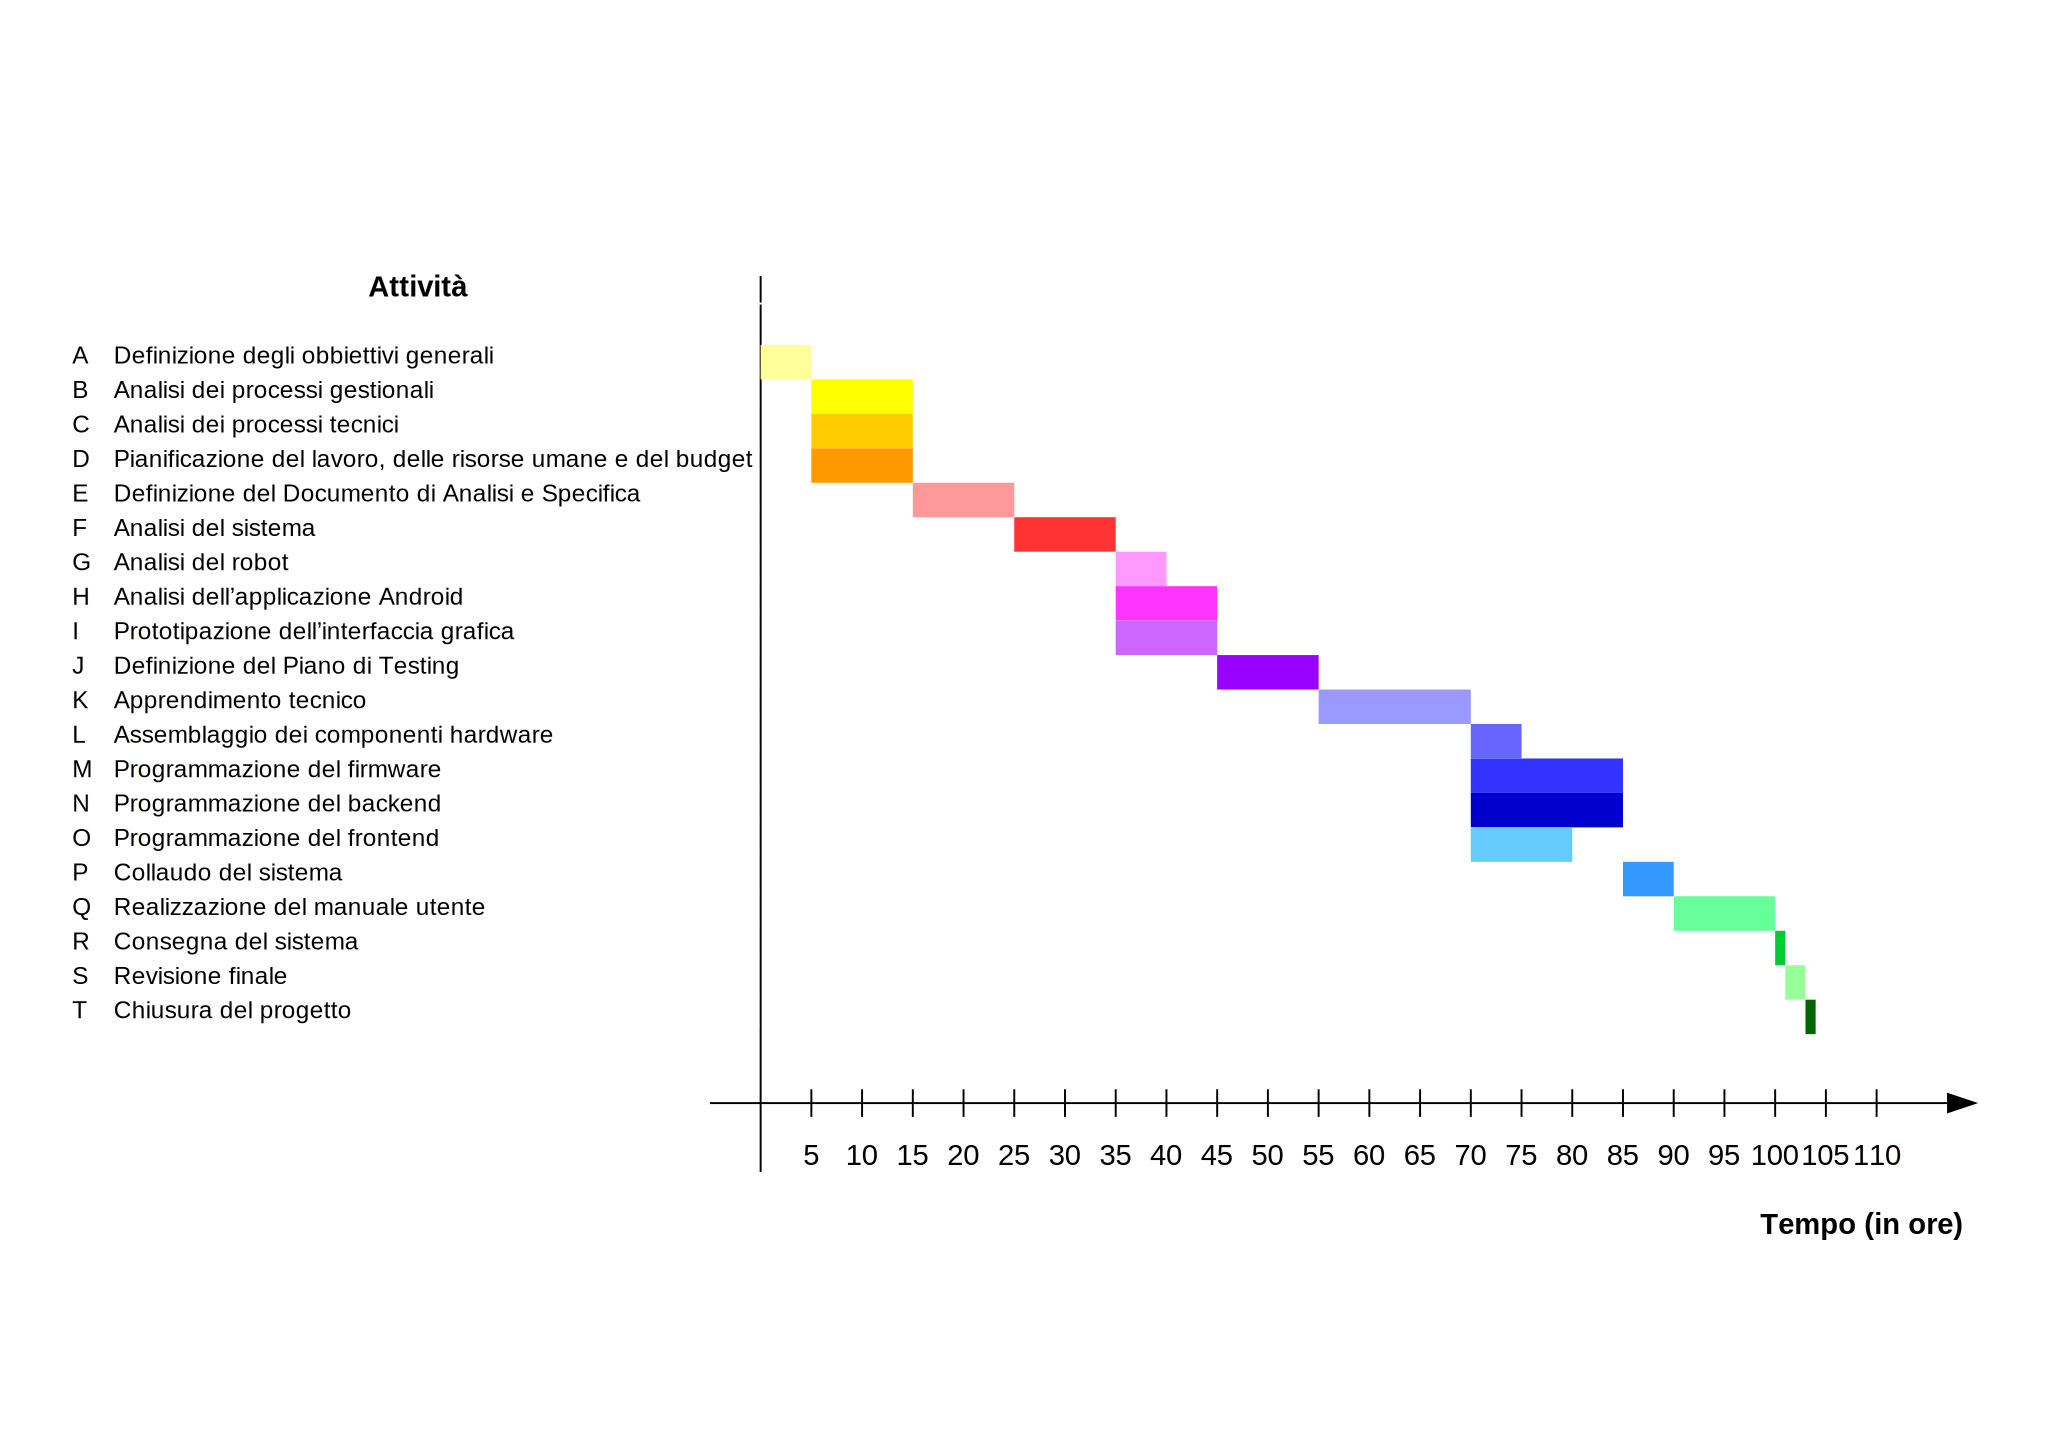
\includegraphics[trim={0 4cm 0 4cm},clip,width=16cm]{Gantt.pdf}
  \caption{Diagramma di Gantt}
  \end{figure}
  
  \begin{figure}[htbp]
  \centering
  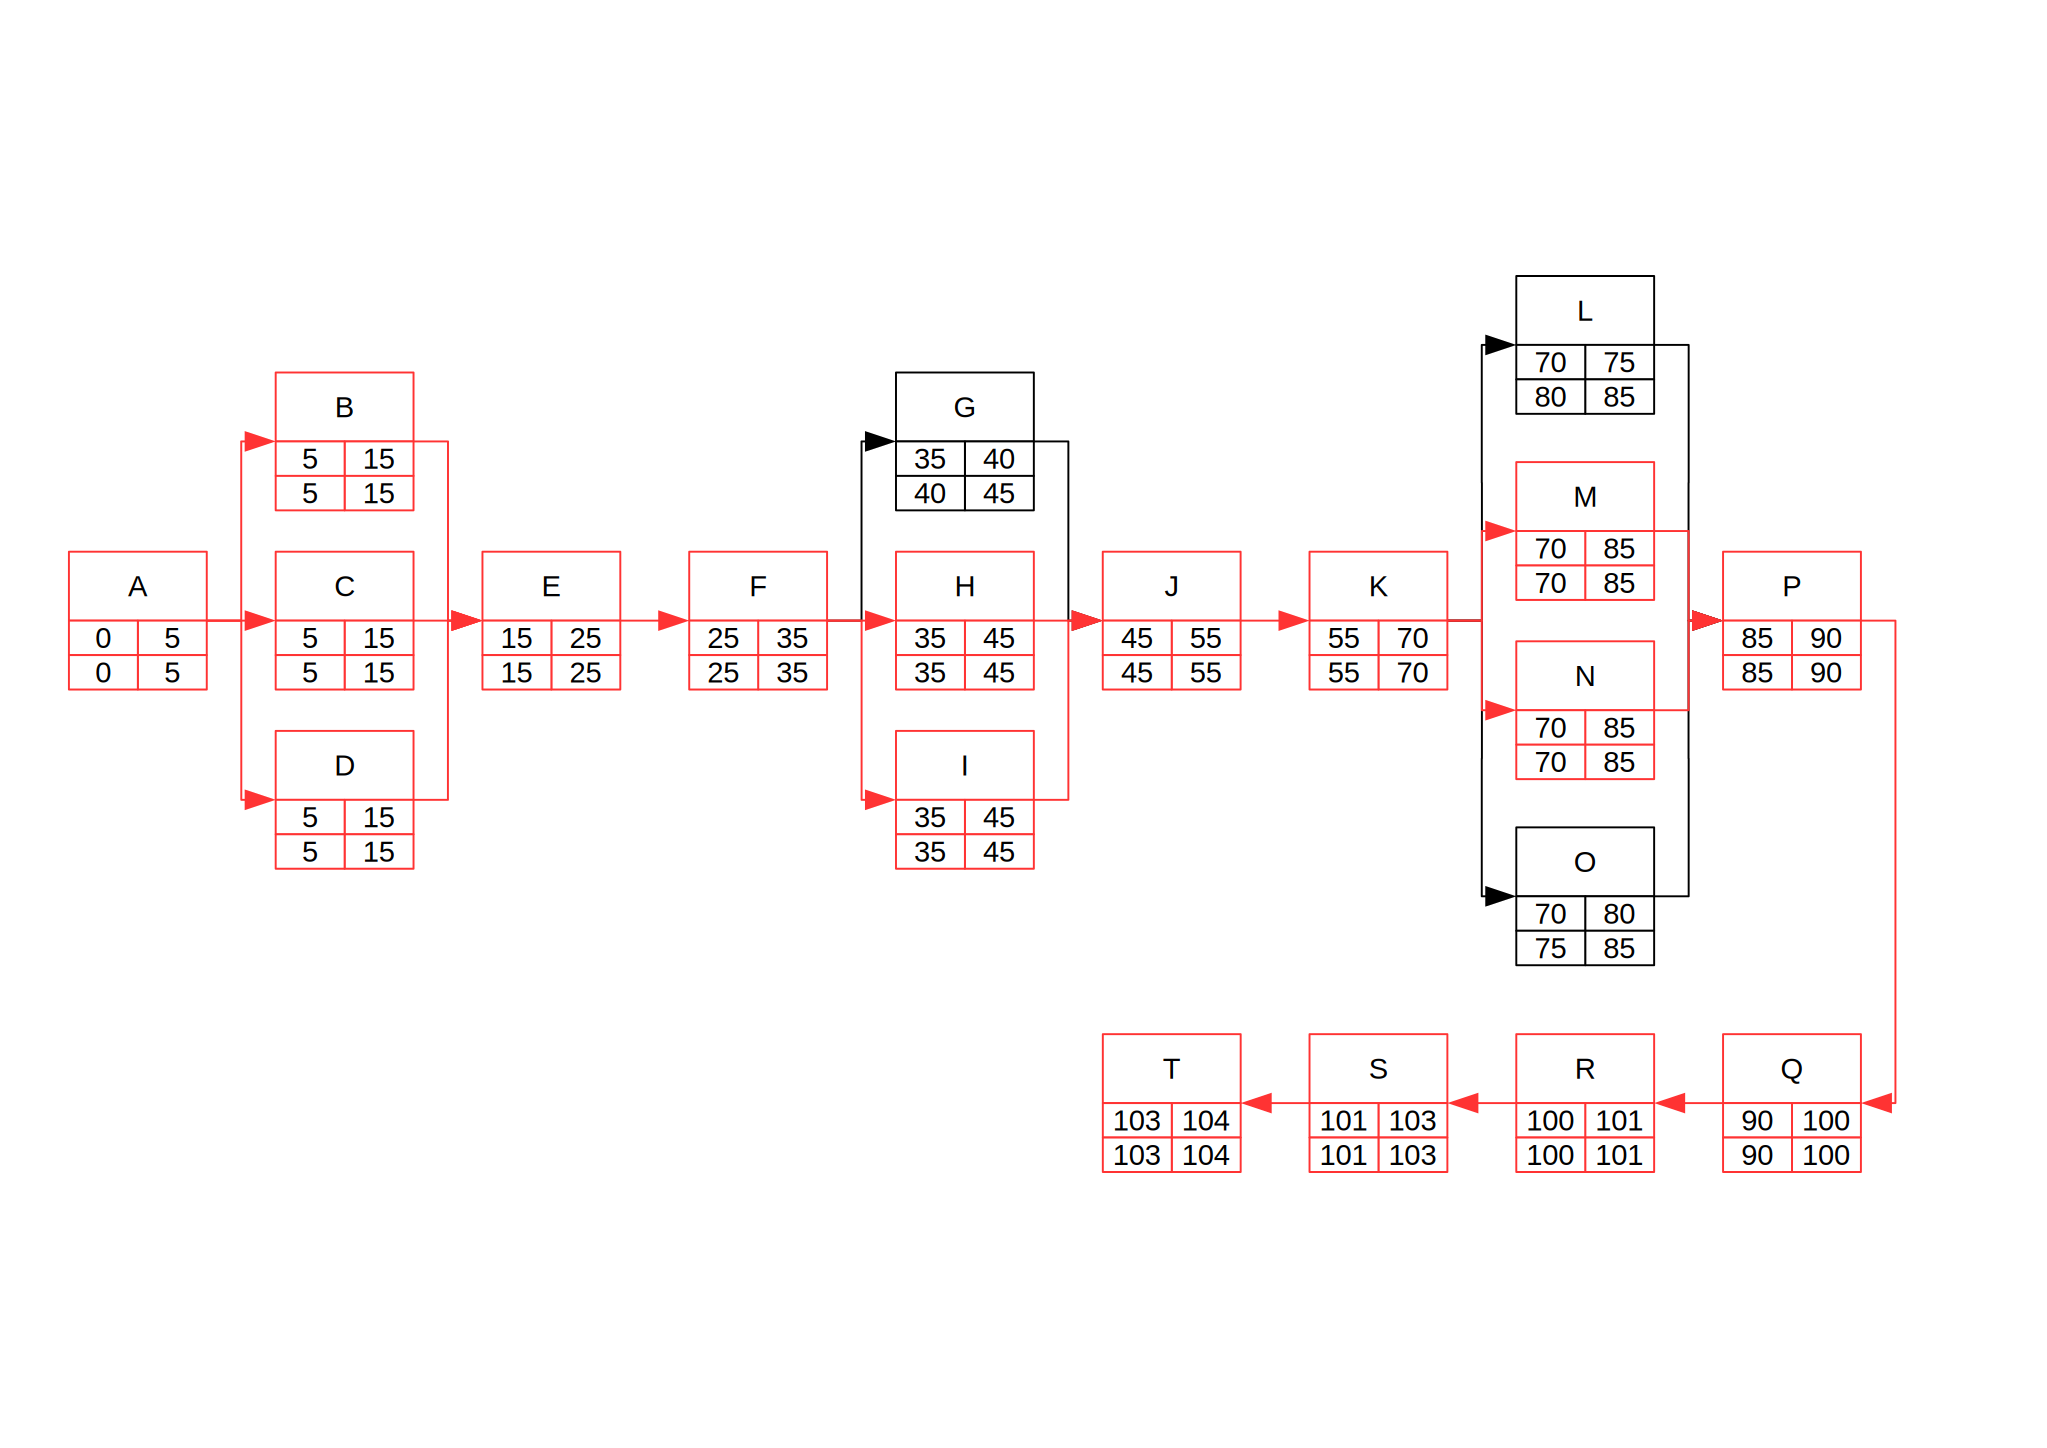
\includegraphics[trim={0 4cm 0 4cm},clip,width=16cm]{PERT.pdf}
  \caption{Diagramma di Pert}
  \end{figure}
  
  
  \subsection{Risorse necessarie}
  
  Le risorse necessarie per la realizzazione del progetto sono: -
  
  \begin{itemize}
  \item \textbf{Risorse umane}: i membri del team di sviluppo e testing e i responsabili di gestione progetto;
  \item \textbf{Risorse hardware}: un computer connesso ad Internet per ogni membro del team, hardware necessario per il robot;
  \item \textbf{Risorse software}: \emph{Telegram} (comunicazione), \emph{Discord} (comunicazione), \emph{GitHub} (gestione delle versioni del progetto), \emph{Typora} (stesura della documentazione), \emph{Latex} (impaginazione della documentazione), \emph{gcc} (compilazione firmware), \emph{CMake} (automazione della compilazione), \emph{VSCode} (programmazione del firmware), \emph{Android Studio} (programmazione dell'applicazione Android).
  \end{itemize}
  
  \subsection{Allocazione del budget e delle
  risorse}
  
  Lo sviluppo dell'applicazione non richiede alcun tipo di risorsa
  economica, in quanto i software impiegati per la realizzazione sono a
  costo zero. Inoltre, anche il set Lego Mindstorms EV3 è stato fornito in
  comodato d'uso dall'Università Ca' Foscari.
  
  Eventuali sensori esterni saranno acquistati dai componenti del progetto
  in maniera volontaria e indipendente e non saranno considerati nel
  budget di progetto.
  
  \subsection{Pianificazione}
  
  La pianificazione del progetto è basata sui termini di consegna del
  progetto e di tutta la relativa documentazione, stabiliti con il
  professor Cortesi all'interno del corso di Ingegneria del Software
  2018/2019:
  \begin{itemize}
  \item Piano di Progetto: 16/10/2018
  \item Documento di Analisi e Specifica: 02/11/2018
  \item Piano di Testing: 15/11/2018
  \item Documento di Progettazione: 10/12/2018
  \item Realizzazione e messa in linea: 31/01/2019
  \end{itemize}
  
  
  
  \end{document}
  